\chapter{Simulations}\label{ch:results}

This chapter presents four simulation experiments that aim at visualizing some of the theory presented in Chapter \ref{ch:hpfc}. The experiments cover the mapping onto the essential and allowable position space described in \ref{subsec:task-oriented}, the use of various closed kinematic chain formulations described in \ref{subsec:task-restrictions}, the computation of control commands for active joints only described in \ref{subsec:passive-joints}, and lastly the simultaneous control of position and force. All of these experiments are modifications of the dynamic HPFC presented in \ref{subsec:DHPFC}.

In addition to these control experiments, an experiment for validating the physics of the simulator is initially provided. Furthermore, the simulator setup and related limitations are presented to give a general overview of the experiment framework.

\section{Simulator configuration for experiments}\label{sec:sim-config-exp}

All experiments are executed in a sterile simulation environment only containing a frictionless ground, the snake robot and three obstacles. The simulator validation test is performed with a snake robot consisting of 14 links. The snake robot is however shrunk to six links for the remaining experiments. This is because the dynamic HPFC method relies on the computation of the dynamical model of the snake robot. This model is computed using the MATLAB Symbolic Math Toolbox \cite{matlabsymbolic} and MATLAB scripts developed in the previous project of the author \cite{AtussaProsjektoppgp}.

Using the dynamical model of the snake robot is computationally expensive because the matrices for the equations of motion of the snake robot get very large for a large number of links. Furthermore, the MATLAB program is unable to calculate the dynamics of a snake robot with a large number of links within a tolerable time frame. Consequently, the control experiments are performed with a snake robot consisting of six links and five joints.

From the presented theory in earlier chapters it is known that the performance of HOAL in snake robots and generally the dynamic HPFC of snake robots is more ideal for snake robots with a large number of links. The fact that the snake robot consists of six links in the control experiments is therefore a limitation to the experiments. Another limitation is the placement of the obstacles. The computed mathematical model used for the control is calculated for a given obstacle-snake robot configuration. That is, the obstacles are in continuous contact with links 2, 3 and 5 on the right, left and right side respectively.

The initial configuration of the snake robot is the same for all experiments, which is a stretched out position along the x-axis, starting in the origin. The joint angles do however deviate slightly from zero as a result of the physics simulator pushing the snake robot away from the static obstacles. This byproduct is probably also contributing to the encountered unsteady force sensor data from the snake robot. The initial configuration of the six link snake robot and the obstacles is shown in Figure \ref{fig:init-gazebo}. The green and blue lines in this figure are indications of axes and viewing angle in the simulator and can be ignored both here and in following simulator captures.
%The advantage of the slight joint angle adjustment is however that the singular start configuration is avoided. \hl{dobbelsjekk plis} 

\begin{figure}[h!]
    \centering
    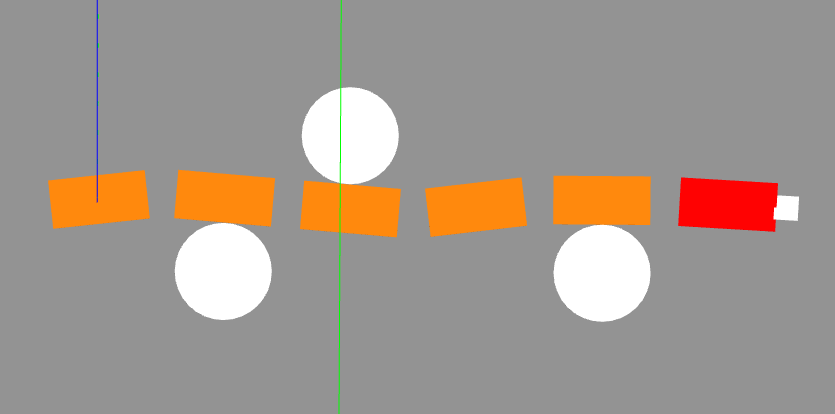
\includegraphics[width=0.6\textwidth]{figures/experiments/initial-gazebo.png}
    \caption{Initial snake robot configuration for dynamic HPFC experiments}
    \label{fig:init-gazebo}
\end{figure}

The control experiments are all based on the dynamic HPFC from \ref{subsec:DHPFC}. The modifications and control structure for the different experiments are presented in the respective sections. All control goals are chosen as simple values to focus the results on the deployed methods. These desired values describe the force against the obstacles and the angle of links in contact with the obstacles. Only a subset of the variables are chosen to be controlled to their desired value for the different experiments. 

\section{Simulator validity test}

% Purpose of experiments
The purpose of this experiment is to test the performance and validity of the physics engine in the simulator. In particular, the interaction forces arising from contact between the snake and obstacles are studied.

The idea is to control the snake robot to a completely stretched out configuration while obstacles are symmetrically placed in contact around its center. At the same time, the snake robot should apply a constant motor torque to the center link. The obstacles are placed in a manner that prevent the joint from getting displaced. In order to still stay stretched out, all other joints will have to apply a torque calculated by the joint PID controller.

The simulator configuration for this experiment is summarized in Table \ref{tab:exp_valid1}. The link and obstacle specific configurations can be found in \ref{sec:simsetup}.

\begin{table}[h!]
    \centering
    \begin{tabular}{|c|c|c|}
        \hline
        & \textbf{Value} & \textbf{Unit}\\
        \hline \hline
        Number of obstacles & $3$ & \\
        Number of links & $14$ & \\
        Initial joint angles & $\mathbf{0}_{13 \times 1}$ & $[rad]$ \\
        $\tau_7$ & $-2$ & $[Nm]$ \\
        $[K_p, K_i, K_d]$ & $[10, 3, 0.3]$ &\\
        \hline
    \end{tabular}
    \caption{Simulation configuration for simulator validation test}
    \label{tab:exp_valid1}
\end{table}

\begin{figure}
    \centering
    
\includegraphics[width=0.9\textwidth]{figures/experiments/exp_valid1.pdf}
    \caption{Illustration of validation test}
    \label{fig:valid1_sketch}
\end{figure}

The placement of the obstacles and snake robot is illustrated in Figure \ref{fig:valid1_sketch}. As can be observed from the figure, the two outermost obstacles will establish a counter force to the resulting force from the middle joint motor torque. The resulting joint torques from this scenario are expected to comply with the well known relationship
% Math stuff
\begin{equation}
    \tau = r\times f,
\end{equation}
where $r$ is the distance from the force origin to the joint.

Since all joints are separated with equal distances and the snake robot is completely stretched out, it is expected that the torques follow a linear relationship with respect to their placement from the center. In addition, since the obstacles are symmetrically placed around the center of the robot, it is expected that the torque values are symmetrical around the center joint as well.

\begin{figure}[h!]
    \centering
    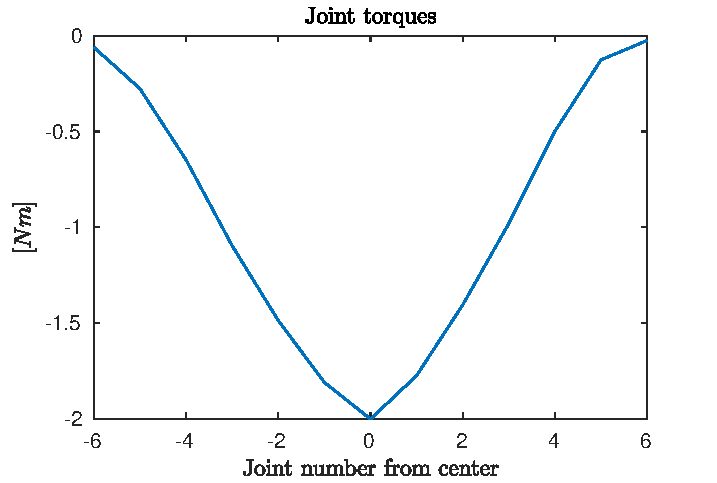
\includegraphics[width=0.9\textwidth]{figures/experiments/validation1.pdf}
    \caption{Snake robot joint torques from simulator validation test}
    \label{fig:validation1}
\end{figure}

The resulting joint torques are plotted in Figure \ref{fig:validation1}. The x-axis of this plot describes the joint number from the center joint. In order to retrieve the joint torques from the static state part of the simulation, the data was recorded after the snake robot and controller had settled into a steady state.

From the figure it is obvious that the joint torques have a close to symmetrical and linear relationship. The fifth and sixth joints from the center are exceptions here. That is however also expected since they are not between the outer and middle obstacles. A reason for why the graph is not completely linear or symmetrical is probably that it depends on the exact positioning of the obstacles and robot, and this might change slightly after the motor torques are applied. In addition, it depends to a large degree on the controllers effort to "stretch" out the snake robot. From studying Figure \ref{fig:valid1_gazebo} it is possible to see that the snake robot is ever so slightly bent.
Regardless, this experiment is considered to have validated the interaction force computations of the simulator successfully. 

\begin{figure}[h!]
    \centering
    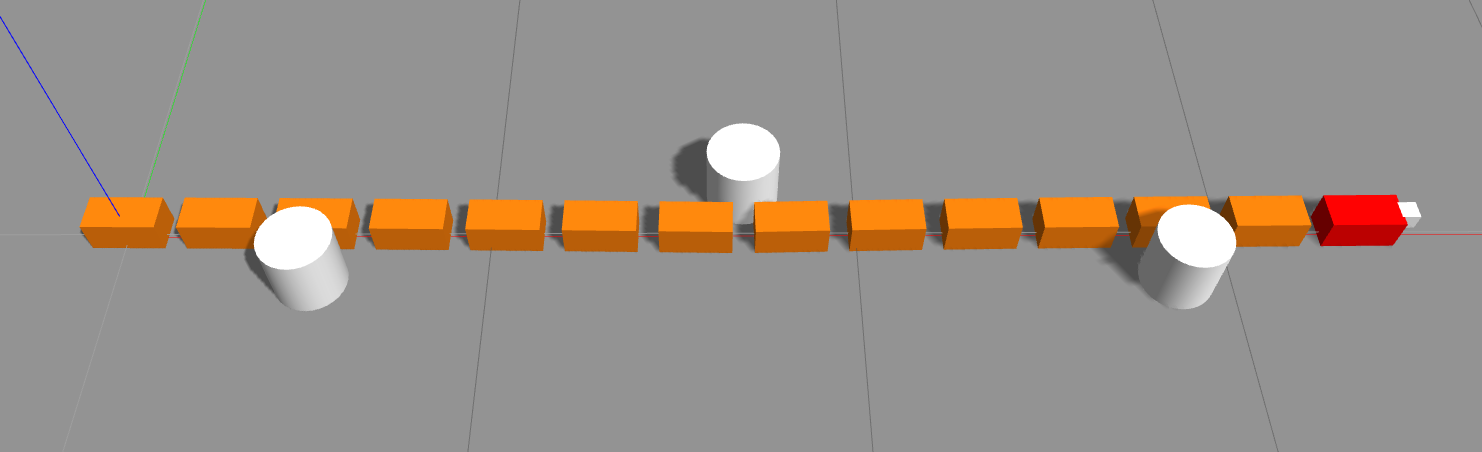
\includegraphics[width=0.9\textwidth]{figures/experiments/exp_valid1_gazebo.png}
    \caption{Screenshot from validation test Gazebo simulation}
    \label{fig:valid1_gazebo}
\end{figure}

\section{Essential position control}\label{sec:ess-pos}

This experiment covers reference following for the angle of a link in contact with an obstacle. The motivation is to show the impact of the mapping to the joined essential and allowable position space. More specifically, the use of the filter $\prescript{}{j}{\mathbf{F}}_{p}$ from (\ref{eq:hpfc_fp}) is studied. This method is also described in more detail in \ref{subsec:task-oriented}.

Link number 5, which is in contact with the foremost obstacle, is controlled to a constant angle $\theta_{t,d,3}$ measured with respect to the base frame. The controlled variable is referred to as $\theta_{t,3}$, and is the only essential variable the filter takes into account in this example. A simulation without the filter is also included to show the importance of defining which variables are essential for a given task when the total number of task variables is greater than the number of actuated joints.

\begin{table}[h!]
    \centering
    \begin{tabular}{|c|c|c|}
        \hline
        & \textbf{Value} & \textbf{Unit}\\
        \hline \hline
        Number of obstacles & $3$ & \\
        Number of links & $6$ & \\
        $\theta_{t,3,d}$ & $0.3$ & $[rad]$ \\
        $[K_p, K_i]$ & $[0.05, 0.005]$ &\\
        Essential variables & $[\theta_{t,3}]$ & $[rad]$ \\
        \hline
    \end{tabular}
    \caption{Simulation configuration for position control experiment}
    \label{tab:exp_single_pos}
\end{table}

The setup for this experiment is presented in Table \ref{tab:exp_single_pos}. It should be noted that the force control is left out. This can also be seen in the control diagram of the experiment presented in Figure \ref{fig:diag-p}. The position filter is included in the diagram, although it is only active for the first simulation of the experiment.

\begin{figure}[H]
    \centering
    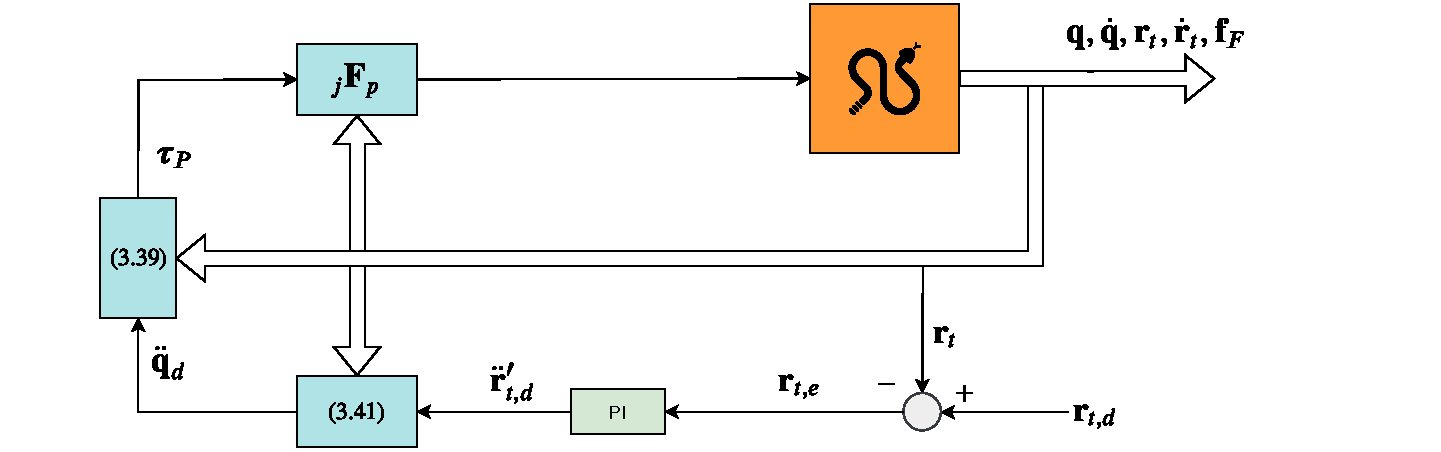
\includegraphics[trim=1cm 0cm 3cm 0cm, clip=true, width=\textwidth]{figures/experiments/control-diagrams/p-control-diagram.pdf}
    \caption{Control diagram for essential position control}
    \label{fig:diag-p}
\end{figure}

The global contact link angle, joint angles and joint torques from the experiments are presented in Figures \ref{fig:singlepos} and \ref{fig:singlepos-nofilter}. As one could imagine, the latter figure shows the unfiltered control case. The contact link is in this case quite far from reaching its reference and the control does not seem to be very purposeful. The corresponding joint angle values show that the snake simply turns its first actuated joint, resulting in the tail of the snake robot spinning around before getting stuck. The behavior of the snake robot in the filtered example makes more sense, as it simply bends the joint preceding to the link and compensates by bending the following joint in the opposite direction.

The configuration of the snake robot at the end of the filtered and unfiltered simulations is better understood by looking at Figures \ref{fig:singlepos-gazebo} and \ref{fig:singlepos-gazebo-nofilter} respectively. From the last figure it is also evident that the robot has lost contact with some of the obstacles, which means that the mathematical model the controller is based on no longer is valid. This is likely to have contributed to the strange control sequence.

\begin{figure}
    \centering
    
    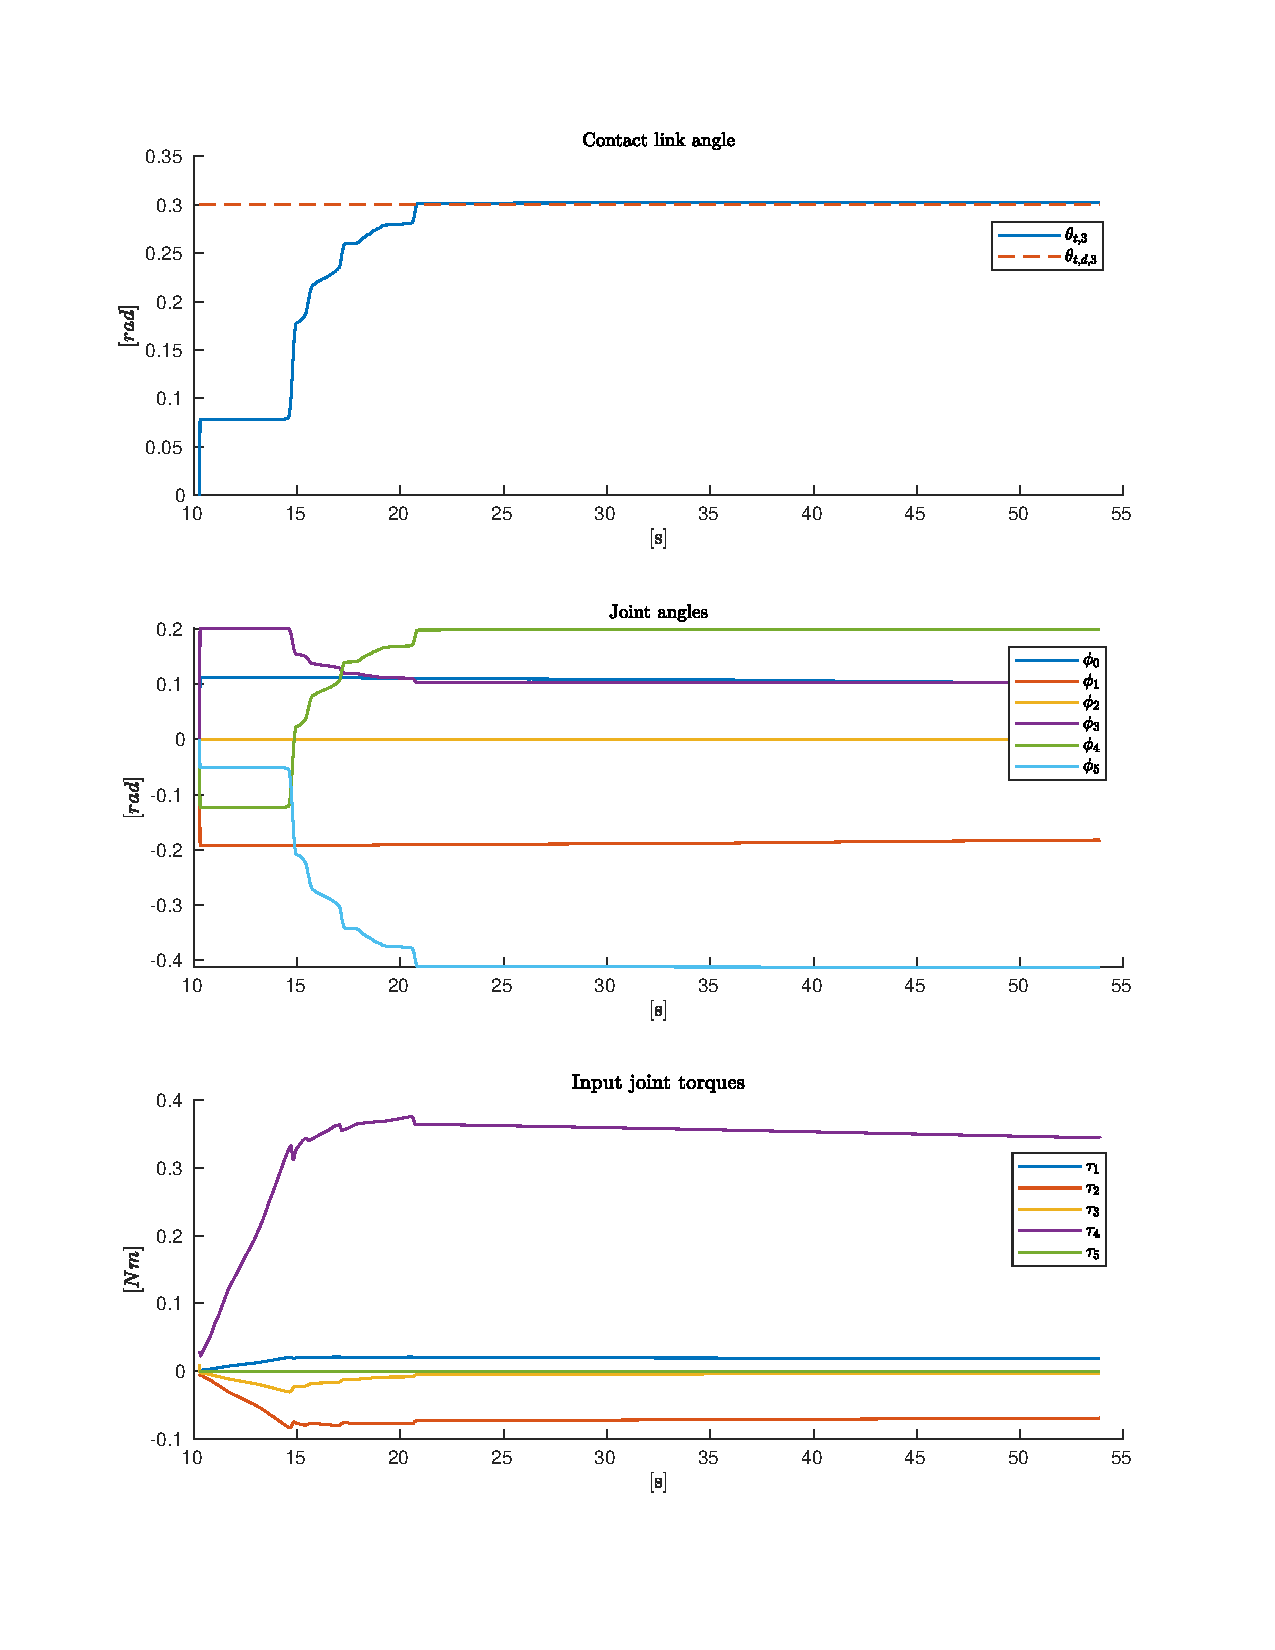
\includegraphics[trim=2cm 2cm 2cm 2cm, clip=true, width=\textwidth]{figures/experiments/single_pos/single-pos-3plot.pdf}

    \caption{Results from filtered position control}
    \label{fig:singlepos}
\end{figure}

\begin{figure}
    \centering
    
    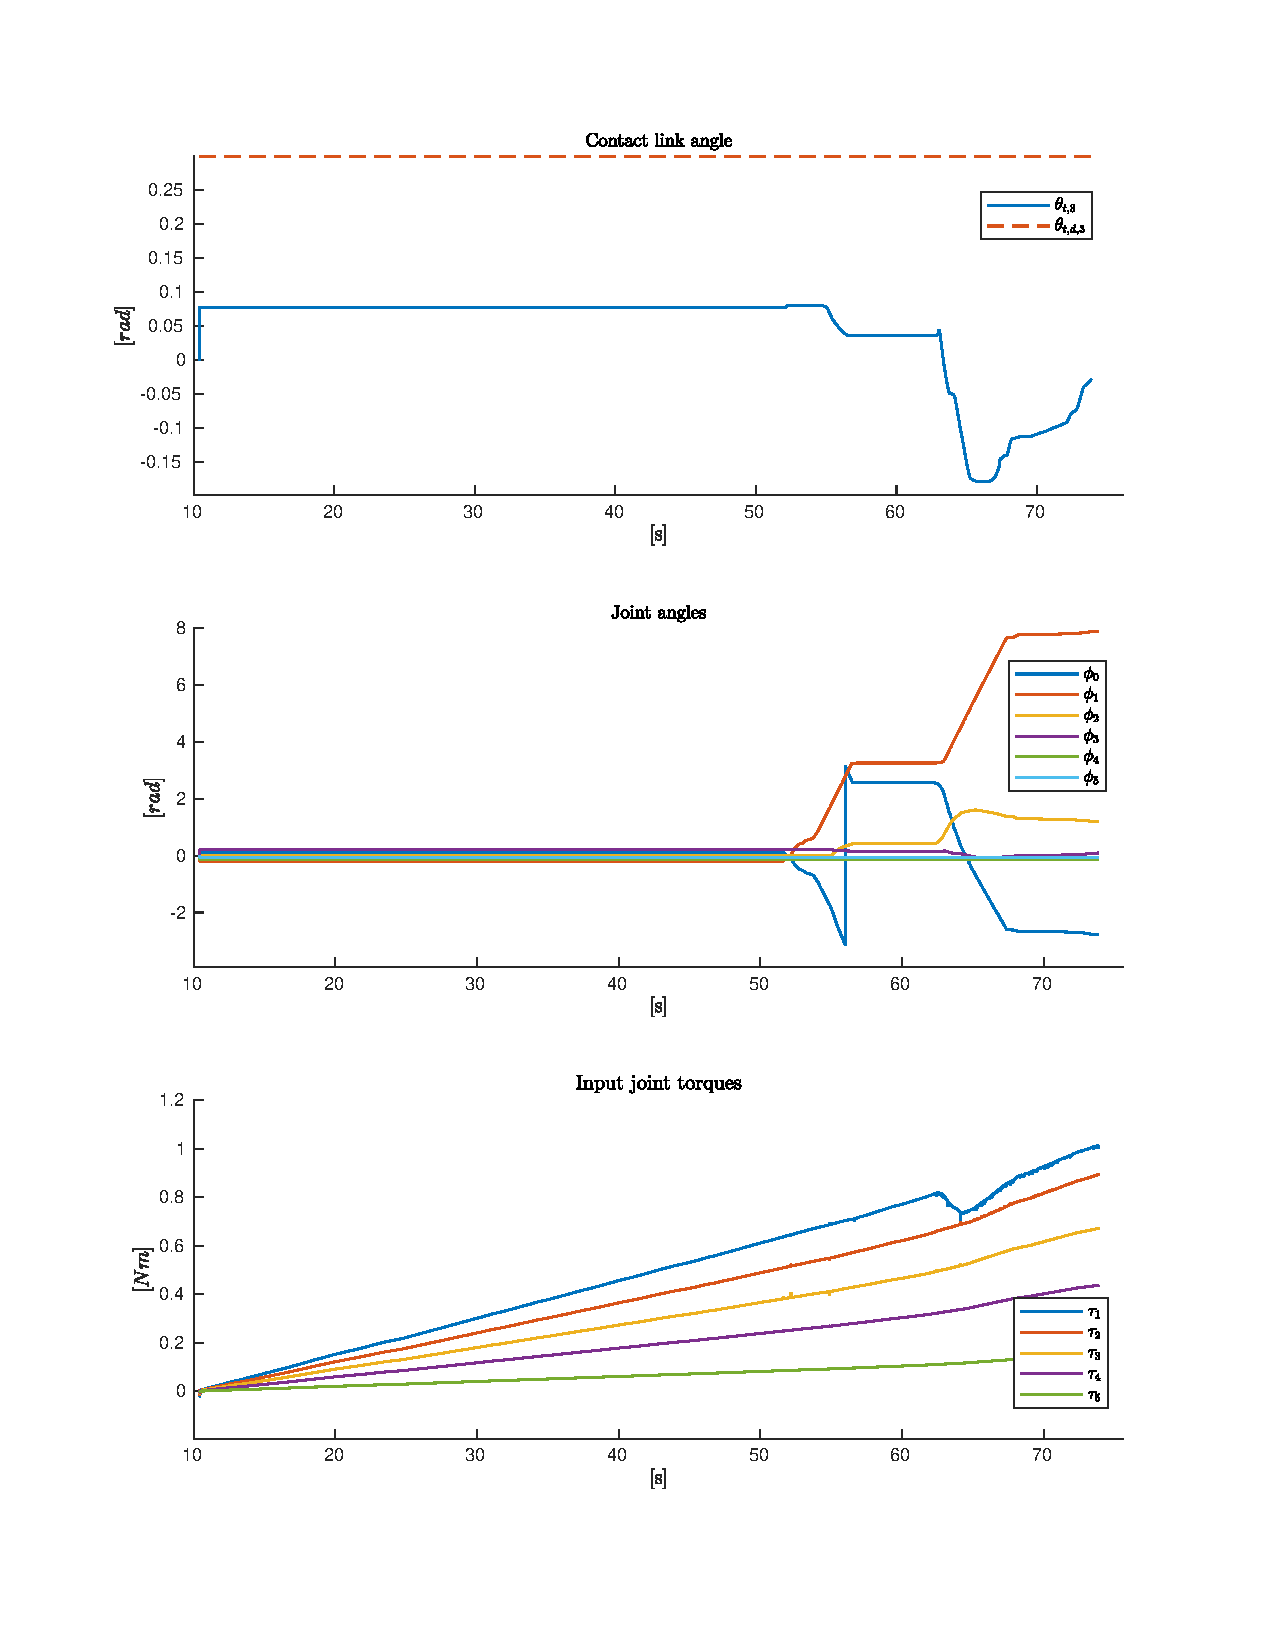
\includegraphics[trim=2cm 2cm 2cm 2cm, clip=true, width=\textwidth]{figures/experiments/single_pos/single-pos-3plot-fail.pdf}

    \caption{Results from unfiltered position control}
    \label{fig:singlepos-nofilter}
\end{figure}

\begin{figure}
    \centering
    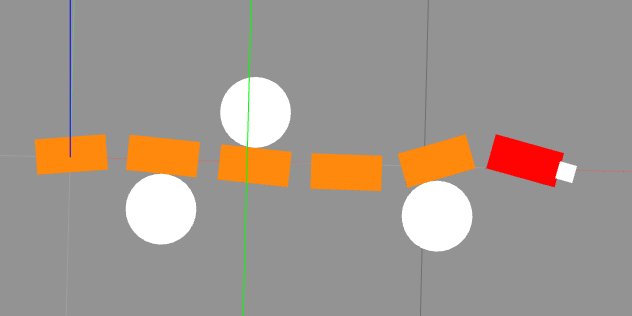
\includegraphics[width=0.5\textwidth]{figures/experiments/single_pos/gazebo_single_pos.png}
    \caption{Snake robot after filtered position control}
    \label{fig:singlepos-gazebo}
\end{figure}

\begin{figure}
    \centering
    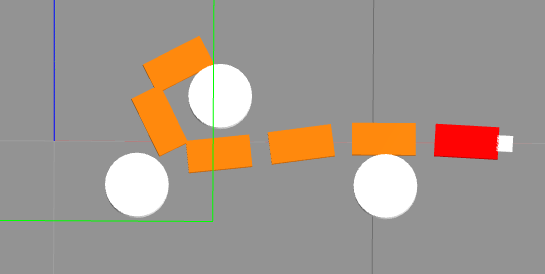
\includegraphics[width=0.5\textwidth]{figures/experiments/single_pos/gazebo_single_pos_nofilter.png}
    \caption{Snake robot after unfiltered position control}
    \label{fig:singlepos-gazebo-nofilter}
\end{figure}
\clearpage
The explanation of the presented results is that the unfiltered case tries to control all possible position variables in $\mathbf{r}$, meaning all contact link angles and the translational position along every contact point. This sums up to 6 variables. However, the robot only has 5 actuators. Furthermore, the last actuator can not be taken into account since it is located after the last contact point. This results in a total of 4 actuators that may be utilized for the control. 
Needless to say, trying to control 6 variables is infeasible for this snake robot. Increasing the number of joints and links would give it a much better basis for achieving the task.

%In this snake robot one can find a total of 6 closed kinematic chains. Three from the base of the robot to the three obstacles and three between the obstacles. That is, one from the first to the second obstacle, one from the first to the third and lastly one from the second to the third. The bottleneck here is the three consecutive closed kinematic chains from the base to obstacle one, from obstacle one to two and two to three. This is because these contain the lowest number of actuated joints. The number of actuated joints in these closed kinematic chains are one, one and two moving forward from the base. This means that two variables could in theory be controlled at the last contact point, but only one on each of the other contact points. 


%It should be noted that the force control is completely left out in this experiment. 





\section{Force control with various CKC formulations}\label{sec:2xminiJforce}

The purpose of this experiment is illustrating the differences between the use of the two closed kinematic chain (CKC) formulations described in \ref{subsec:task-restrictions}. The first simulation is run with minimal CKCs, and the second one is run with the regular CKCs defined with respect to the base frame.

\begin{table}[h!]
    \centering
    \begin{tabular}{|c|c|c|}
        \hline
        & \textbf{Value} & \textbf{Unit}\\
        \hline \hline
        Number of obstacles & $3$ & \\
        Number of links & $6$ & \\
        $f_{F,d}$ & $2$ & $N$ \\
        $[K_{p}, K_{i}]$ & $[0.5, 0.003]$ &\\
        \hline
    \end{tabular}
    \caption{Simulation configuration for force control experiment}
    \label{tab:exp_2xf}
\end{table}

The snake robot is in contact with three obstacles, whereas the force against the second and third obstacle is controlled. The desired force magnitude $f_{F,d}$ is 2 $N$ for both contacts. The simulation configuration is summarized in Table \ref{tab:exp_2xf} and is common for both simulations. The control structure for this experiment is given in Figure \ref{fig:diag-f}.



\begin{figure}[h!]
    \centering
    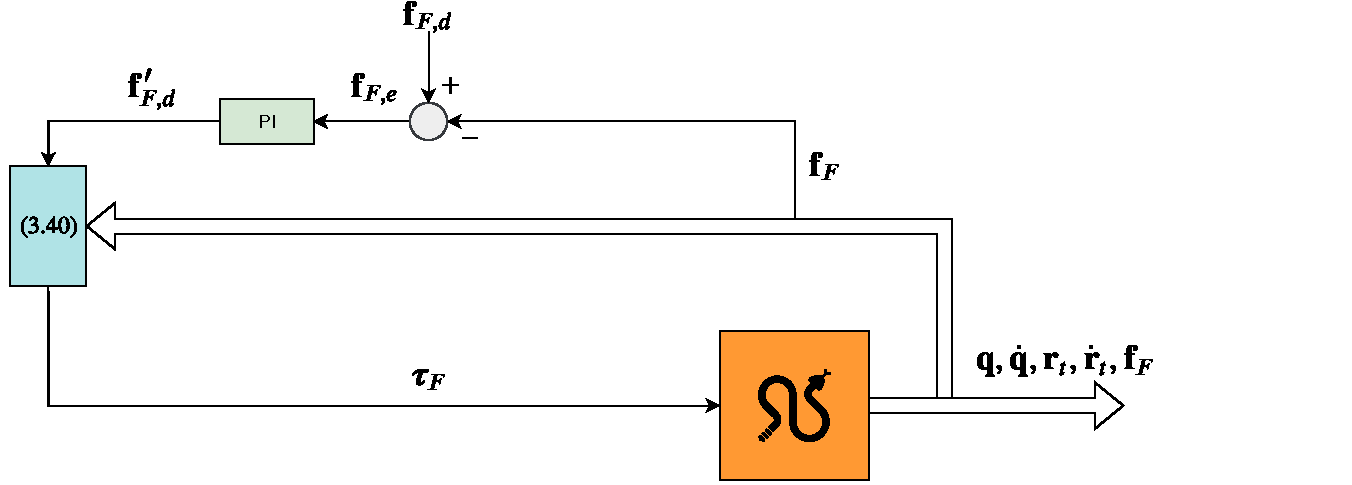
\includegraphics[trim=0cm 0cm 3cm 0cm, clip=true, width=\textwidth]{figures/experiments/control-diagrams/2f-control-diagram.pdf}
    \caption{Control diagram for force control}
    \label{fig:diag-f}
\end{figure}

It should be mentioned that very thorough tuning of control parameters could improve the results of both simulations, although a great deal of tuning already has been conducted. Furthermore, the control is quite twitchy as a result of the unsteady force sensor feedback. The experiment in \ref{sec:pos-force-control-exp} is conducted with a low pass filtering of these sensor signals, and proves that the control consequently gets smoother as well.

\newpage
\subsection{Regular CKCs}

For the first simulation, the regular CKC formulations are used. By regular it is here meant that all contact points are described with respect to the base frame of the robot. This setup is illustrated in Figure \ref{fig:CKC1} in \ref{subsec:task-restrictions}. It can be seen that the two CKCs for the second and third obstacle are overlapping. As a result, the first two joint motors will be carried out to control both contact points. The motors for joints 3 and 4 will however still be reserved the third contact point. From the input torque plot in Figure \ref{fig:2xf-bigJ} it can be seen that all joint motors except for the last one are actuated. The last one is left out as it is positioned after both controlled contact points. 

Figure \ref{fig:2xf-bigJ} also shows the resulting contact forces. As expected, the contact force for the third contact point is much better controlled than for the second contact point. This is because it has more actuators available, again making it more robust. In addition, it is known that the actuators used for the second contact point are shared for both controls. The input torques $\tau_3$ and $\tau_4$ used only for the third contact are clearly much more stable than the shared input torques $\tau_1$ and $\tau_2$.

Another reason for why $f_{F,2}$ never reaches its desired value can be that the joint torques related to this control reach the saturation limit, which has an absolute value of 2 in this experiment. Unfortunately, it was found that larger motor torques easily led to the contact being lost at some moments. This is highly undesired as the mathematical model assumes contact at all times.

\begin{figure}[H]
    \centering
    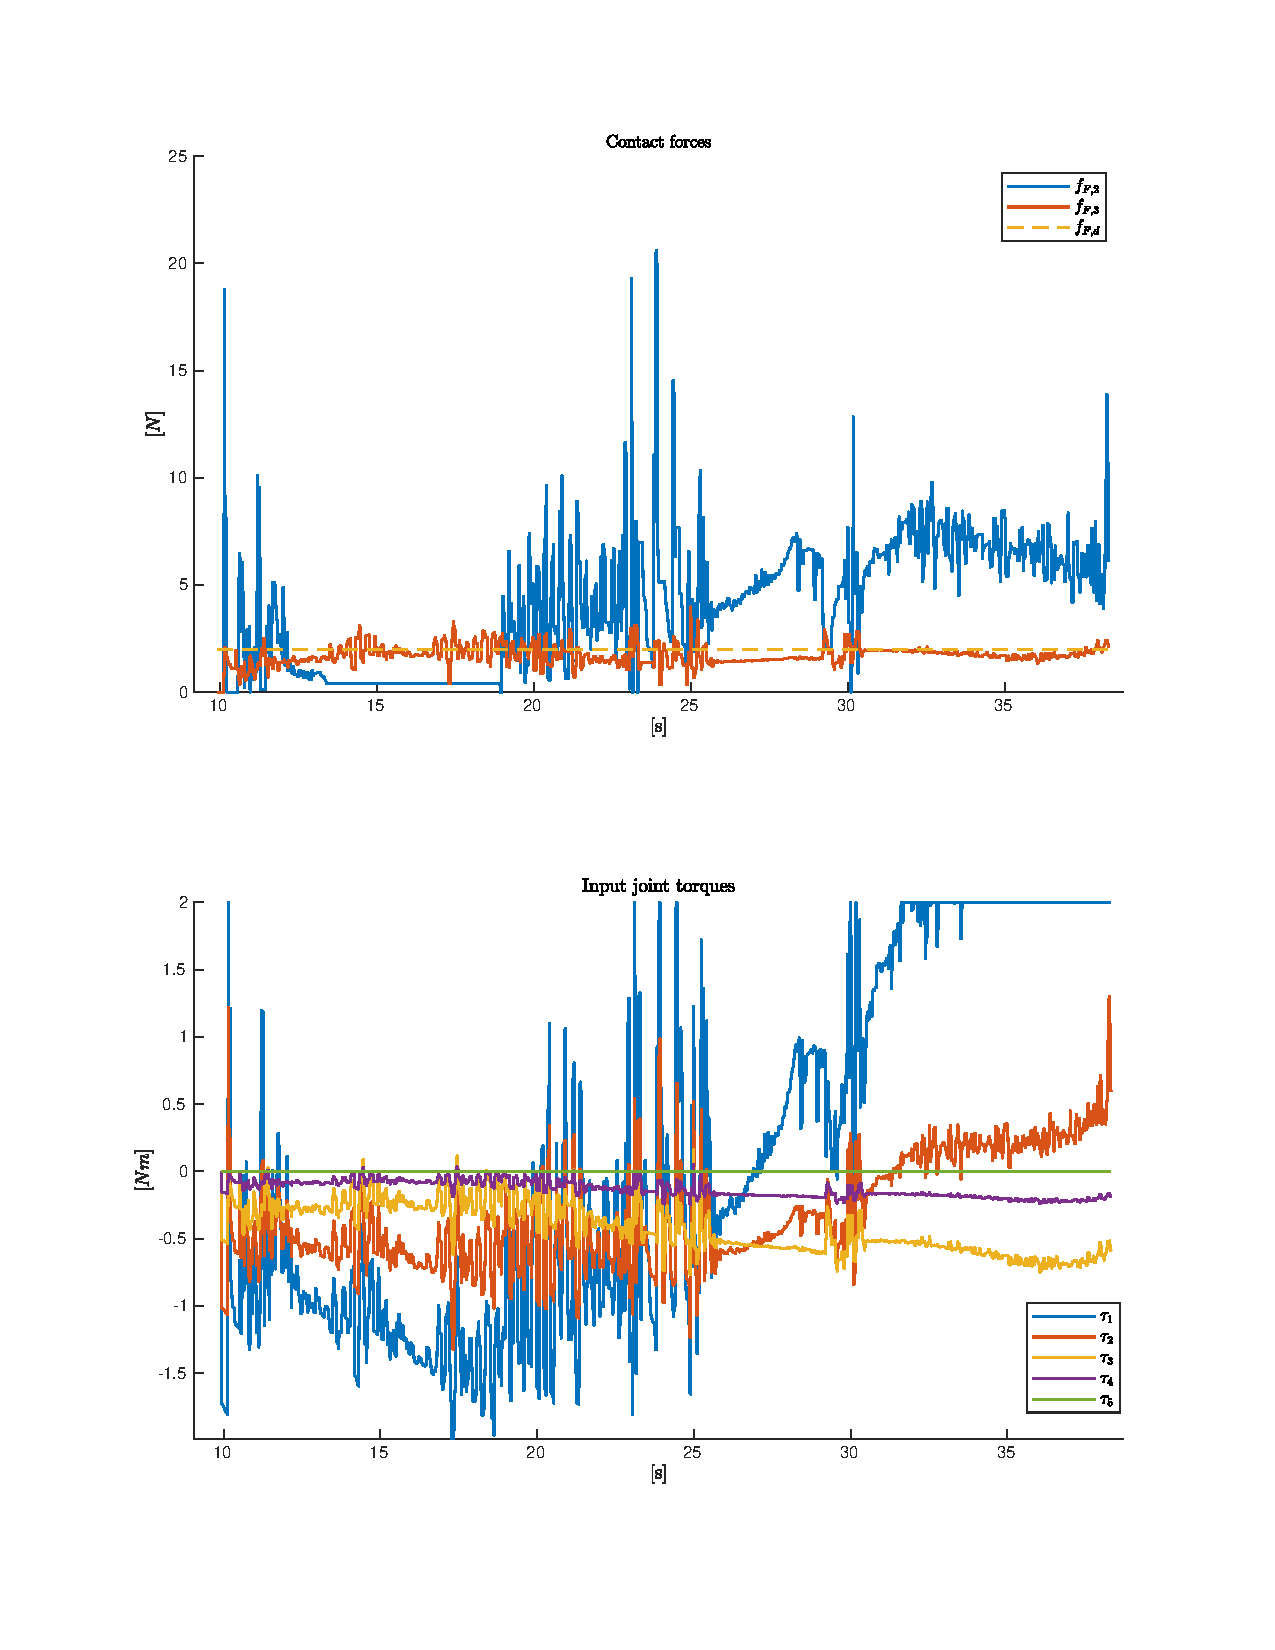
\includegraphics[trim=2cm 2cm 2cm 2cm, clip=true, width=\textwidth]{figures/experiments/2xf/bigJ-2plot.pdf}
    \caption{Results from experiment with regular CKCs}
    \label{fig:2xf-bigJ}
\end{figure}

\subsection{Minimal CKCs}

For the second simulation, the minimal CKC formulations are used, meaning that the CKC for the second obstacle is defined from the first to the second obstacle point, and the CKC for the third obstacle is defined from the second to the third obstacle. This formulation is easier understood from Figure \ref{fig:CKC2} in \ref{subsec:task-restrictions}. It can be observed that the CKC belonging to the third obstacle contains two joints, whereas the second one only contains one joint.

Figure \ref{fig:2xf-miniJ} shows the resulting contact forces and joint torques from the simulation. It can be observed that both forces are close to the desired value. Nonetheless, the force $f_{F,3}$ against the third obstacle is considerably more stable than the force $f_{F,2}$ against the second obstacle. It is not implausible that this is a result of the third contact point having one more joint available for control. This increases the robustness of the control. In addition, it is known that the joint connecting link 3 and 4 will influence the third link. This can further be seen as a disturbance on the control of the second contact force.

From the control torques in Figure \ref{fig:2xf-miniJ}, it is evident that only the motors on joints 2, 3 and 4 are used. This is logical, as it is exactly what the corresponding CKCs allow. Since the controllability increases with the current minimal CKC formulation, the control is also significantly smoother than in the previous simulation.

\begin{figure}[H]
    \centering
    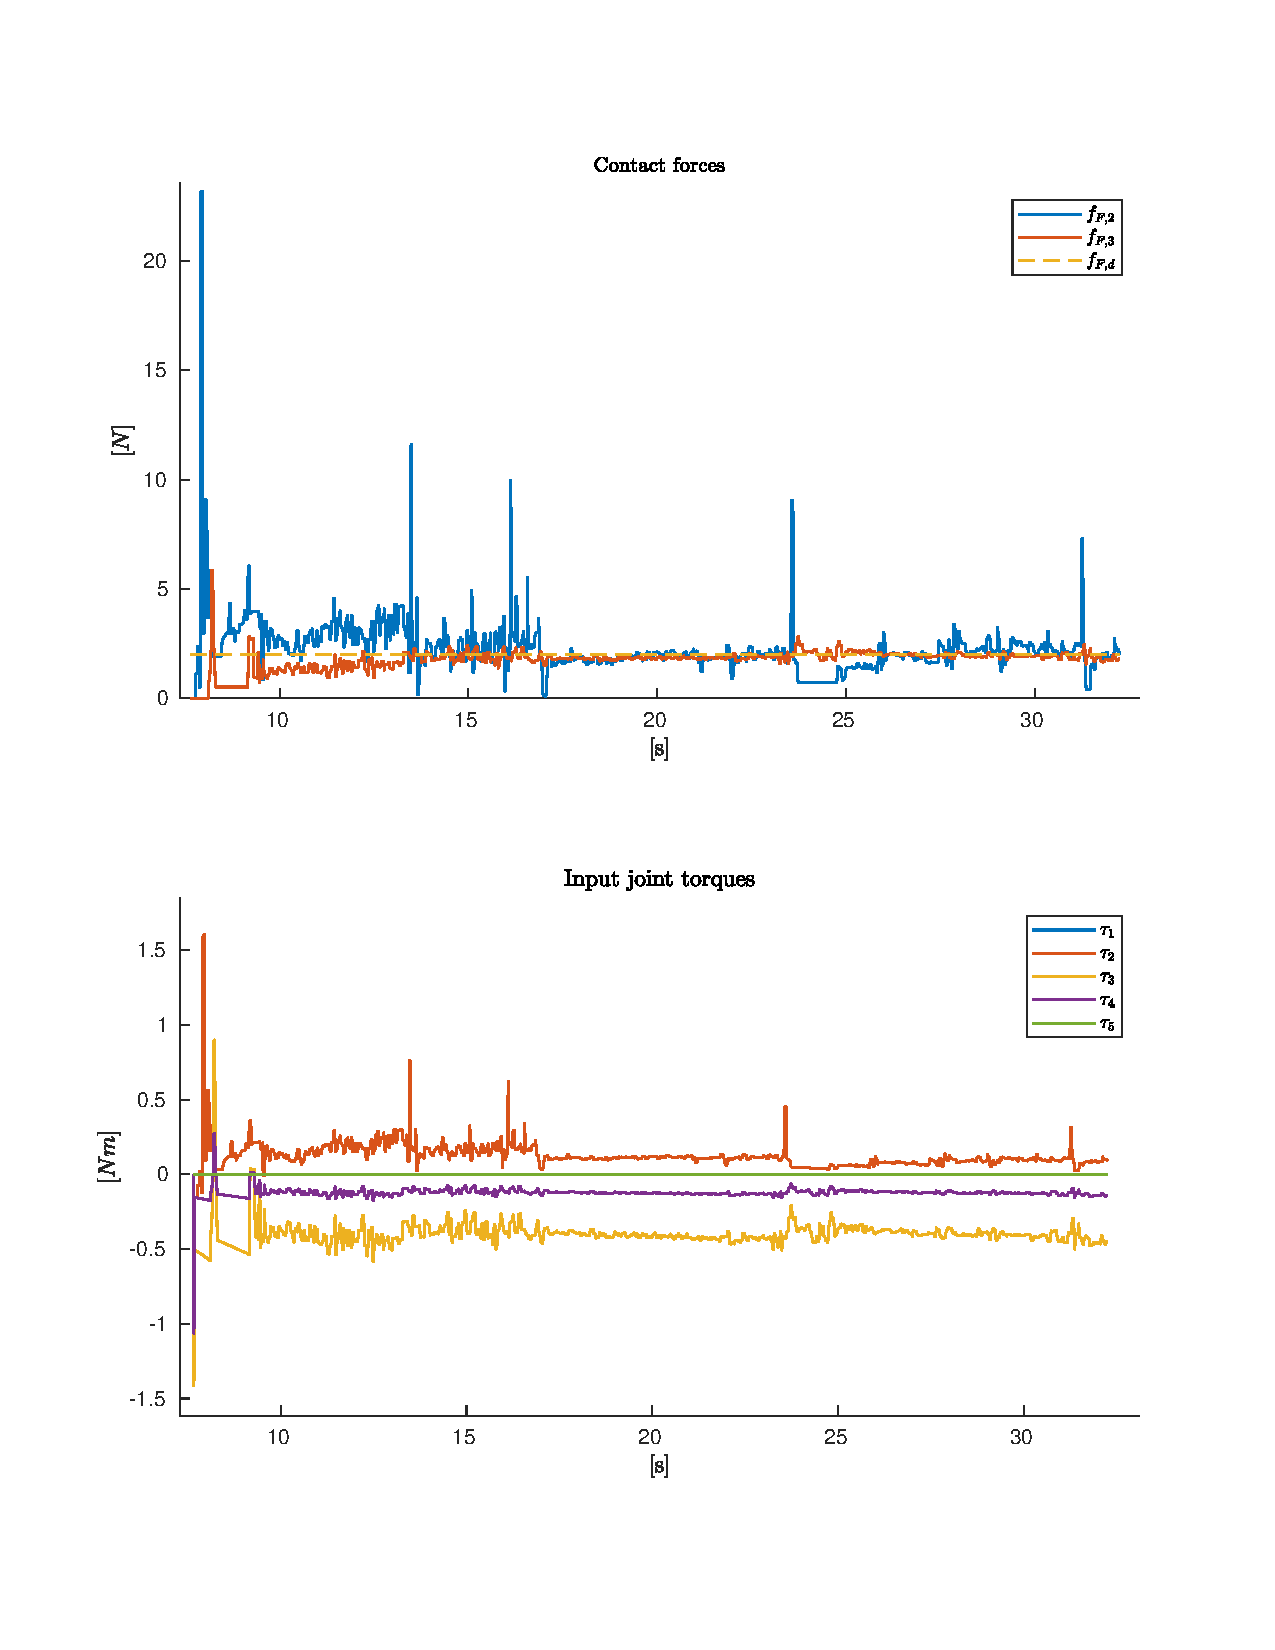
\includegraphics[trim=1.5cm 2cm 2cm 2cm, clip=true, width=\textwidth]{figures/experiments/2xf/miniJ-2plot.pdf}
    \caption{Results from experiment with minimal CKCs}
    \label{fig:2xf-miniJ}
\end{figure}


%Filtering the sensor signals with a low pass filter could have improved the smoothness of the results. However, the main sense of the experiment is still communicated with the presented results.



\section{Position control with active joint torque focus}\label{sec:pas-pos}

As seen in \ref{subsec:DHPFC}, the equations of motion are used to find the desired torques satisfying the desired joint accelerations. However, the equations of motion do not consider that some of the joints are passive and will assign joint torques to all joints, both passive and active. This is of course an issue since the computed solution relies on these torques being realised.

This experiment aims at illustrating the difference in just ignoring the passive joint torque commands and in mapping all joint torques over to the active joints. Because the focus is on the position torques $\boldsymbol{\tau}_P$, the link angle by the second and third obstacle is controlled. It is first controlled only by using the equations of motion as in (\ref{eq:dhpfc_taup}). Here the torques for the passive joints are simply neglected. The second simulation shows control where all torques are mapped to the active joints, as explained in \ref{subsec:passive-joints}. For this experiment it was simply chosen that the desired values of the active joints should be followed and that the passive joints could take resulting arbitrary values. This is probably not the optimal choice of variables to control, but no method for determining this has to this point been developed. The matter is discussed further in \ref{}.

The minimal CKC formulation is used for both simulations, which implies that the desired angles are defined according to the previous contact point. Further simulation configurations are presented in Table \ref{tab:exp_2xp}. The control structure for the experiment is given in Figure \ref{fig:diag-2p}. The equation (\ref{eq:tau-act}) is substituted with (\ref{eq:dhpfc_taup}) for the first simulation.

\begin{table}[]
    \centering
    \begin{tabular}{|c|c|c|}
        \hline
        & Value & Unit\\
        \hline
        Number of obstacles & $3$ & \\
        Number of links & $6$ & \\
        $\theta_{2,d}$ & $-0.2$ & $rad$ \\
        $\theta_{3,d}$ & $0.2$ & $rad$ \\
        First sim.:$[K_{p}, K_{i}]$ & $[3, 0.01]$ &\\
        Second sim.:$[K_{p}, K_{i}]$ & $[1, 0.001]$ &\\
        \hline
    \end{tabular}
    \caption{Simulation configuration for force control experiment with minimal CKCs}
    \label{tab:exp_2xp}
\end{table}

\begin{figure}
    \centering
    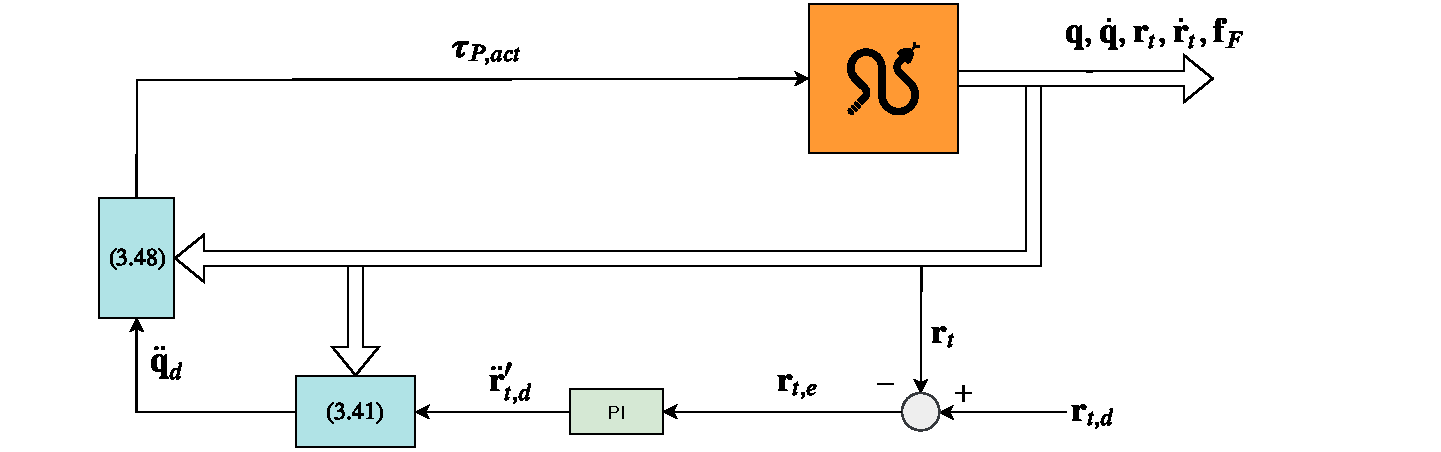
\includegraphics[trim=1cm 0cm 3cm 0cm, clip=true, width=\textwidth]{figures/experiments/control-diagrams/2p-control-diagram.pdf}
    \caption{Control diagram for position control with active joint torque focus}
    \label{fig:diag-2p}
\end{figure}

\subsection{Control torques computed for both passive and active joints}

For this simulation, the control torques from (\ref{eq:dhpfc_taup}) belonging to the active variables were commanded to the snake robot. The rest of the motor torque commands were simply ignored. The resulting torques and contact link angles can be seen in Figure \ref{fig:2xp-1}. The contact link angle $\theta_{t,3}$ settles at a value close to its desired value. However, $\theta_{t,2}$ is very far from reaching its desired value and the control is overall considered unsuccessful.

\begin{figure}[H]
    \centering
    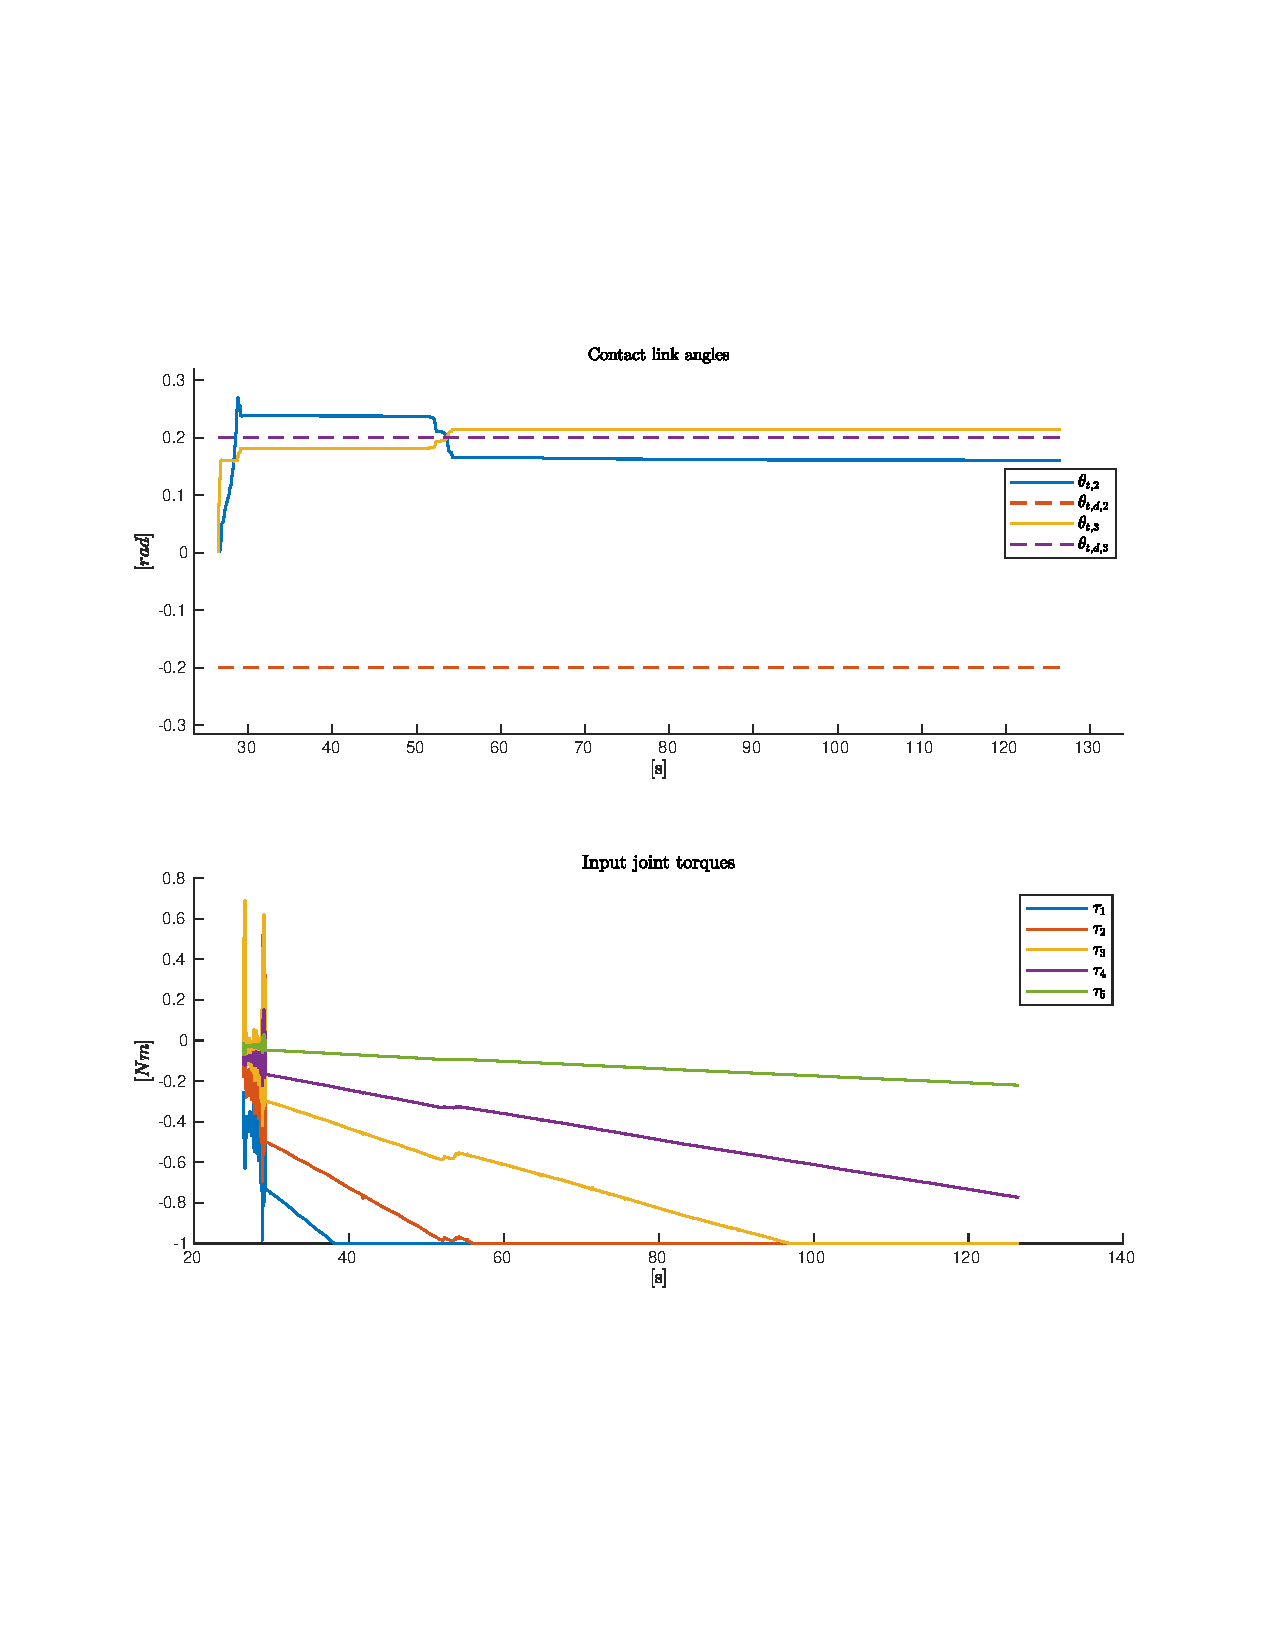
\includegraphics[trim=2.1cm 6cm 2.1cm 5cm, clip=true, width=\textwidth]{figures/experiments/2xpos/2xpos-2plot-fail.pdf}
    \caption{Position control experiment with torque calculation for all joints}
    \label{fig:2xp-1}
\end{figure}

From Figure \ref{fig:2xp-1} it can also be observed that the joint torques reach a saturation limit, which is probably the reason for why very little change is noticed in the angle values. The saturation is in place to keep the snake robot from making large sudden movements that would put it outside of the model validity. A higher saturation limit was also tested without further success. Another reason for the static behavior of the angles is the configuration of the snake robot and obstacles, presented in \ref{}. When all applied joint torques are negative the snake robot will try to curve up towards the two right side obstacles. By doing so it is mainly just pushing against the obstacles, much like the experiment in \ref{tab:exp_valid1}. This will logically not lead to any movement.

\subsection{Control torques computed for only active joints}

This time the control torques are calculated to all be commanded to the active joints, which means that no commands are ignored. The desired passive joint acceleration values are on the other hand ignored, so this is not an optimal approach either and required a lot of tuning to get right. The results are presented in Figure \ref{fig:2xp-2}. $\theta_{t,2}$ still deviates slightly from its desired value $\theta_{t,d,2}$, but the performance is still considered much better than in the previous simulation.

\begin{figure}[H]
    \centering
    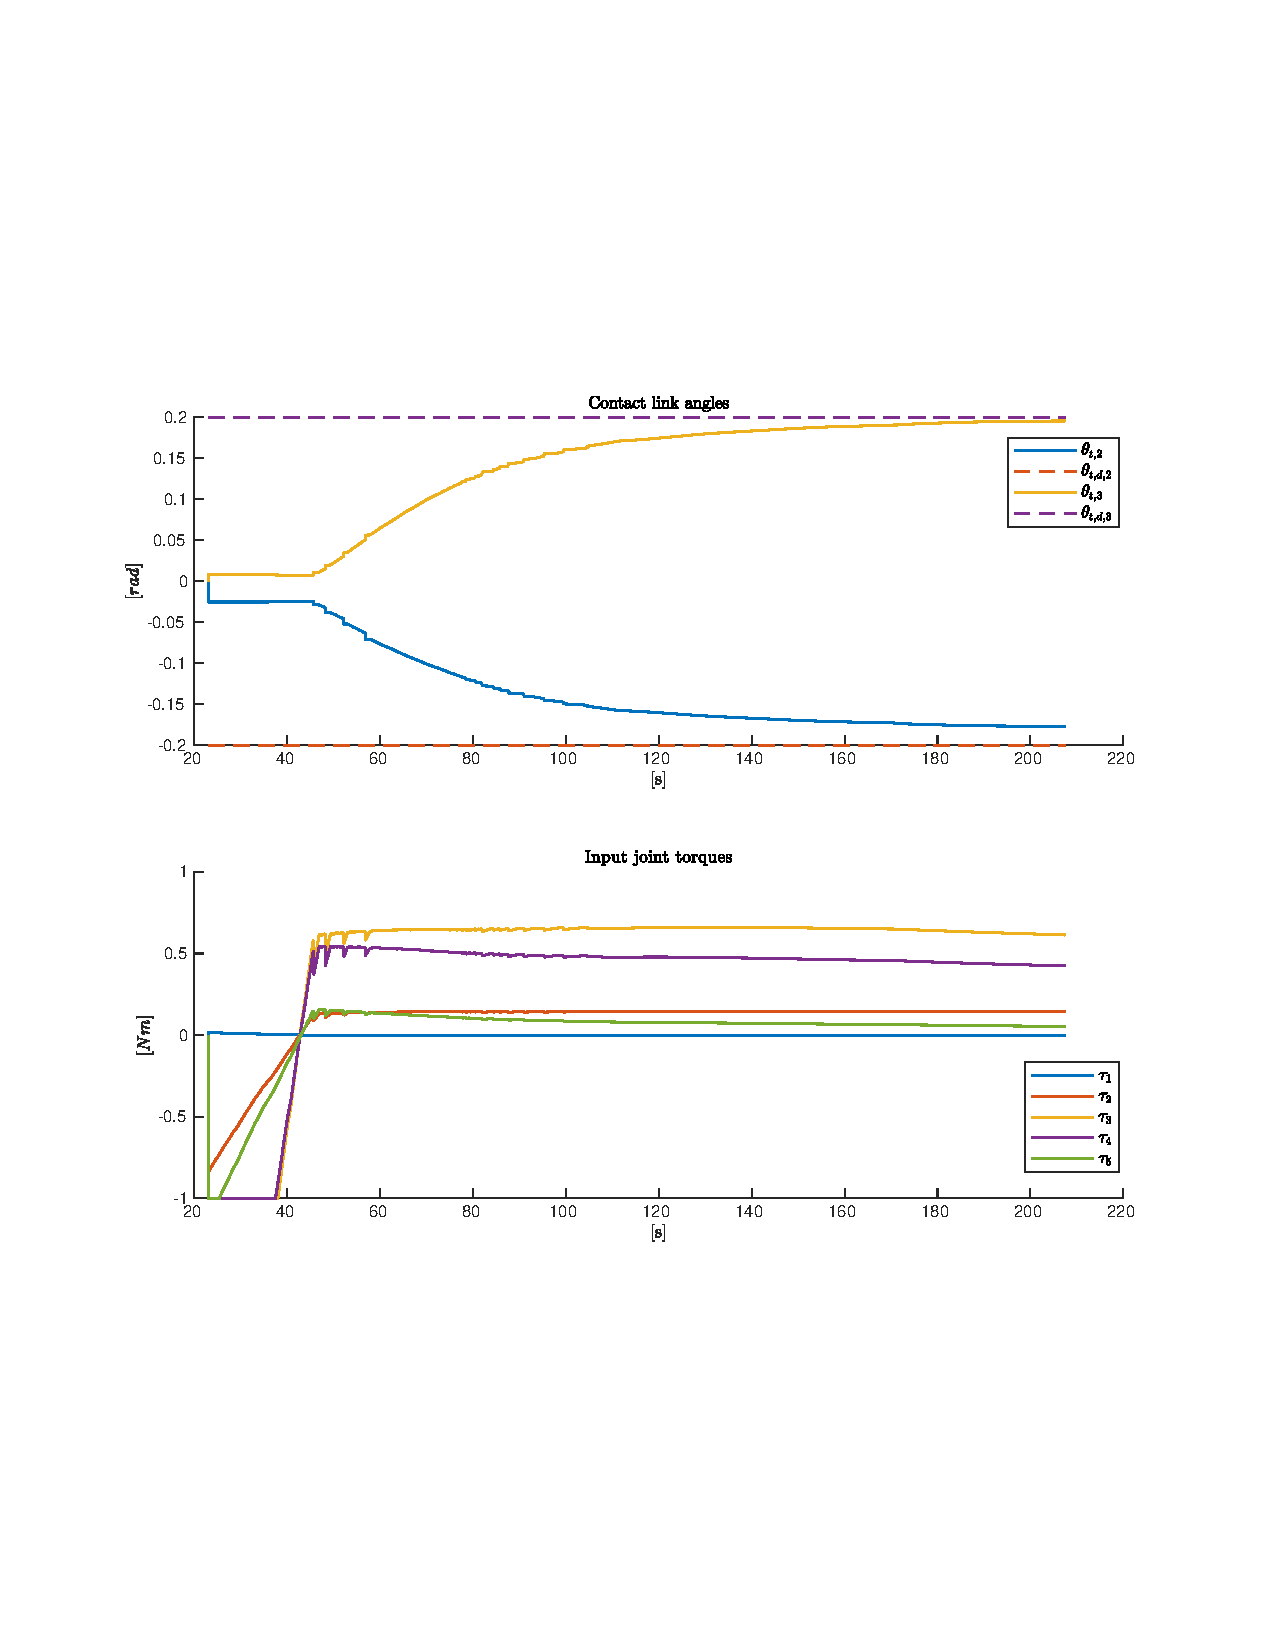
\includegraphics[trim=2.1cm 6cm 2.1cm 6cm, clip=true, width=\textwidth]{figures/experiments/2xpos/2xpos-2plot.pdf}
    \caption{Position control experiment with torque calculation for for only active joints}
    \label{fig:2xp-2}
\end{figure}

It should be noted that the snake robot is moving quite slowly in both of the simulations. This means that $\mathbf{C(q,\dot{q})}$, the part of the dynamics dependent on the joint velocities, is playing a very inessential role here. To research this method more thoroughly, further experiments should be carried out with a larger number of snake robot joints, more rapid movements and last but not least, a more intelligent and reasoned choice of which joints should be precisely controlled.

\section{Simultaneous position/force control}\label{sec:pos-force-control-exp}

This last example combines the explored methods from the previous experiments \ref{sec:2xminiJforce}-\ref{sec:pas-pos}. That means that the minimal CKC formulation explained in \ref{subsec:task-restrictions} is applied, and that the joint torques are computed for only the active joints as explained in \ref{subsec:passive-joints}. The rest of the control method is according to the dynamic HPFC control scheme presented in \ref{subsec:DHPFC}.

\begin{table}[h!]
    \centering
    \begin{tabular}{|c|c|c|}
        \hline
        & \textbf{Value} & \textbf{Unit}\\
        \hline \hline
        Number of obstacles & $3$ & \\
        Number of links & $6$ & \\
        $f_{F,d,3}$ & $1$ & $[N]$ \\
        $\theta_{t,d,3}$ & $0.1$ & $[rad]$ \\
        Force:$[K_{p}, K_{i}]$ & $[1, 0.005]$ &\\
        Position:$[K_{p}, K_{i}]$ & $[3, 0.005]$ &\\
        \hline
    \end{tabular}
    \caption{Simulation configuration for simultaneous position and force control experiment}
    \label{tab:p+f}
\end{table}

In this experiment, both position and force is controlled for the third contact point. More specifically, the angle of the link in contact with the third obstacle and the force this link applies to the obstacle are controlled. The exact desired values, as well as general simulation configurations for the experiment, are given in Table \ref{tab:p+f}. The values were chosen with the intuition of what would be achievable for the snake robot from its initial configuration. The control structure for the simulation is given in Figure \ref{fig:diag-pf}.

\begin{figure}
    \centering
    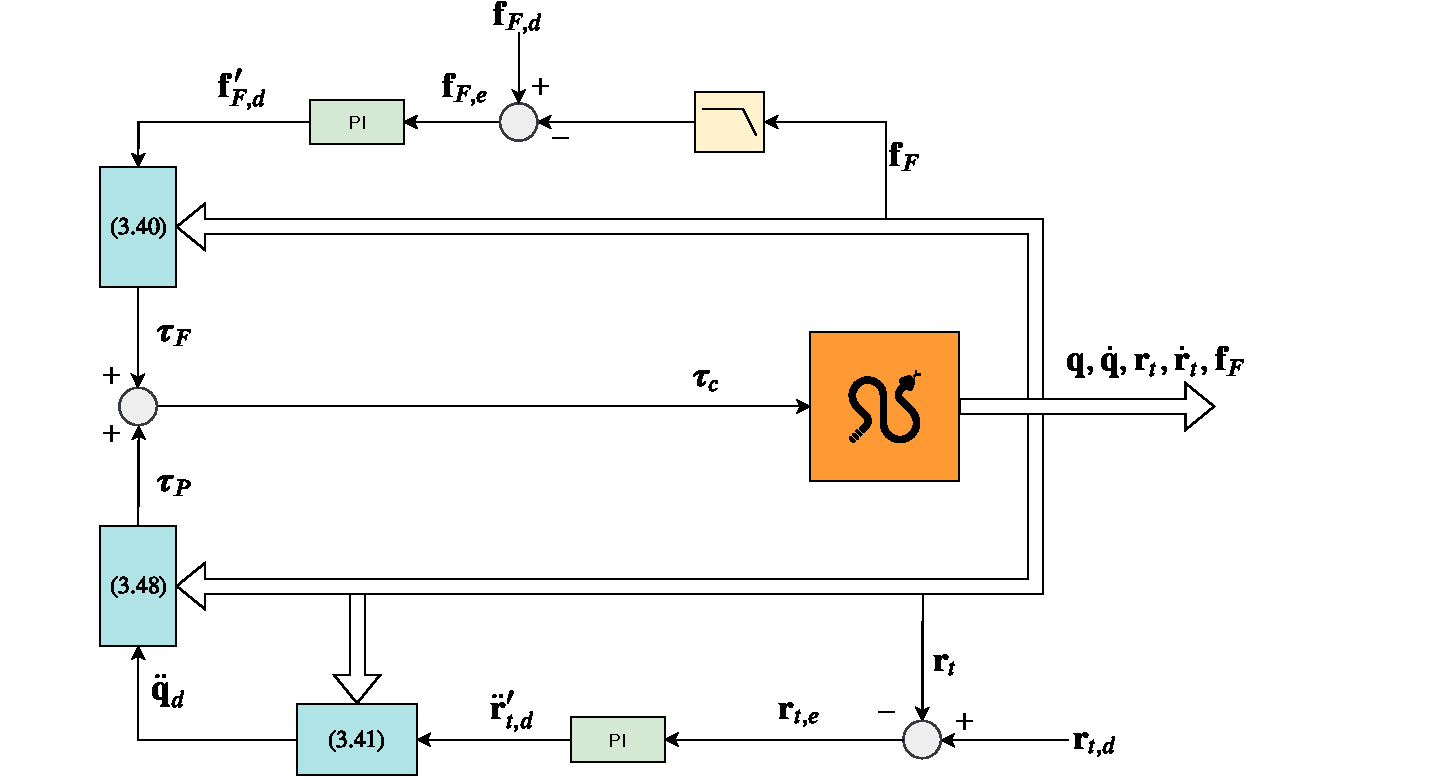
\includegraphics[trim=1cm 0cm 3cm 0cm, clip=true, width=\textwidth]{figures/experiments/control-diagrams/pf-control-diagram.pdf}
    \caption{Control diagram for dynamic HPFC}
    \label{fig:diag-pf}
\end{figure}
\newpage
The resulting contact link angle, contact force and joint torques are presented in Figure \ref{fig:p+f}. In this experiment, the torque values controlling the force are much smoother than the force signal, as opposed to the experiment in \ref{sec:2xminiJforce}. This is because the force sensor signal is filtered before it is sent to the controller. The force signal shown in the figure is unfiltered.

From Figure \ref{fig:p+f} it can also be seen that both the desired angle and force is reached. However, the angle takes longer to reach its reference and does have a slightly irregular trajectory. Both this and the very sensitive force signals can be a result of the nature of the simulator used.
%In addition, since the movements are all over slow, the snake robot ends up stopping and starting frequently, forcing it to also frequently overcome its inertia and suddenly start moving. \hl{yay or nay?}

From the input torque plot in Figure \ref{fig:p+f} it can be observed that the commanded torques $\tau_1$, $\tau_2$ and $\tau_3$ are used only for the position control since they are smoother, whereas $\tau_4$ and $\tau_5$ are used for both position and force control. The idea of Yoshikawa \cite{yoshikawa1987dynamic} is that this can still yield successful HPFC given that the dynamical model is correct. The position and force loops are included to compensate for possible modeling errors.

\begin{figure}
    \centering
    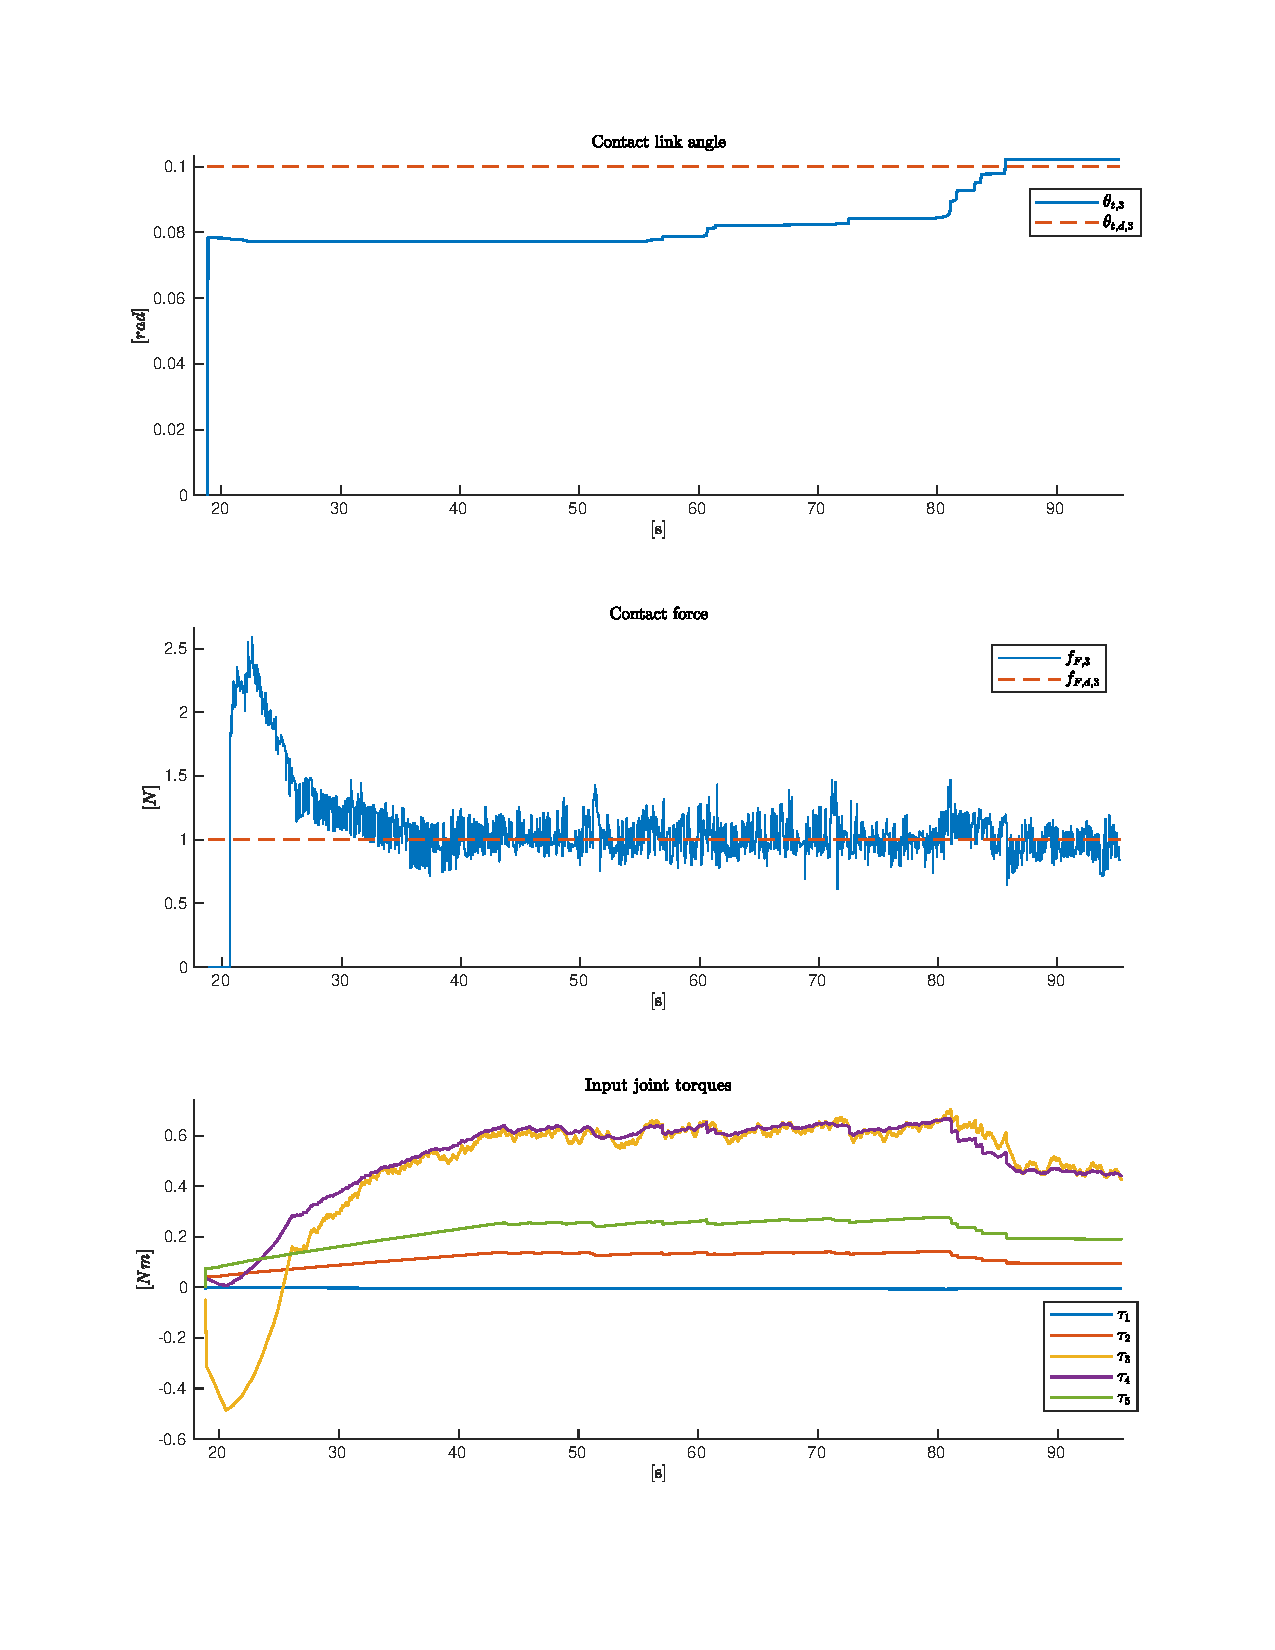
\includegraphics[trim=2.1cm 2.1cm 2.1cm 2.1cm, clip=true, width=\textwidth]{figures/experiments/pos+f/pf-ref-3.pdf}
    \caption{Results from simultaneous force and position control}
    \label{fig:p+f}
\end{figure}